%% ===========================================================================
%%  Informe final - MIA-204 Aprendizaje por Refuerzo
%%  Formato IEEE conference (IEEEtran). Compilar en Overleaf con pdfLaTeX.
%%
%%  Archivo maestro: el contenido está dividido en secciones/*.tex.
%%  Las figuras (PNG) están en figuras/ y se listan en secciones/figuras.tex.
%%  Para regenerarlas: cd ../dqn && python gen_figuras_informe.py
%% ===========================================================================
\documentclass[conference]{IEEEtran}
\IEEEoverridecommandlockouts

\usepackage[utf8]{inputenc}
\usepackage[spanish]{babel}
\usepackage{amsmath,amssymb,amsfonts}
\usepackage{graphicx}
\usepackage{booktabs}
\usepackage{algorithm}
\usepackage{algpseudocode}
\usepackage{url}
\usepackage{hyperref}

% babel-spanish nombra las tablas "Cuadro" y el flotante de algoritmo en inglés.
% El \addto es necesario: babel fija los nombres al empezar el documento.
\addto\captionsspanish{\renewcommand{\tablename}{Tabla}}
\floatname{algorithm}{Algoritmo}

\begin{document}

\title{Navegación de costo mínimo sobre terreno real\\
mediante Aprendizaje por Refuerzo Profundo}

% \author{
% \IEEEauthorblockN{Integrante 1, Integrante 2, Integrante 3,\\ Integrante 4, Integrante 5}
% \IEEEauthorblockA{\textit{Maestría en Inteligencia Artificial (MIA-204)}\\
% \textit{Aprendizaje por Refuerzo}\\
% Arequipa, Perú}
% }

\author{\IEEEauthorblockN{Andres Flores\IEEEauthorrefmark{1};
Victor Lazo\IEEEauthorrefmark{1};
Rubén López\IEEEauthorrefmark{1};
Juan Quispe\IEEEauthorrefmark{1}}
\IEEEauthorblockA{\IEEEauthorrefmark{1}Escuela de Posgrado FIIS - UNI, Lima\\
% \IEEEauthorblockA{\IEEEauthorrefmark{2}Departamento de estudios/ Institución/ Dirección 2\\
E-mail: affloresb@uni.pe, vlazop@uni.pe, ruben.lopez.m@uni.pe, juan.quispe.h@uni.pe}}


\maketitle

% --------------------------------------------------------------------------
\begin{abstract}
En el presente artículo se aborda el problema del aprendizaje de navegación autónoma de costo mínimo sobre topografía real mediante Aprendizaje por Refuerzo Profundo (DRL). A diferencia del enfoque previo basado en Q-learning tabular con condiciones fijas, este trabajo incrementa la complejidad del entorno utilizando un modelo digital de elevación a resolución completa ($108\times108$ celdas de 30~m), donde el agente opera bajo observación parcial y estados iniciales aleatorios en cada episodio. Se aproxima la función de valor de la acción mediante una red Deep Q-Network (DQN) y se realiza una evaluación sistemática comparando métodos basados en valor (DQN y Double DQN) y basados en política (REINFORCE), empleando el algoritmo de Dijkstra como línea base de optimalidad. Los resultados experimentales demuestran la viabilidad de la propuesta: el agente entrenado generaliza con éxito hacia posiciones iniciales no observadas, describiendo trayectorias cercanas al óptimo y mostrando robustez ante transiciones estocásticas. Adicionalmente, se caracterizan y resuelven dos problemas críticos de diseño: el colapso del aprendizaje inducido por el rediseño de recompensa (*reward shaping*) potencial bajo descuento temporal, solucionado mediante un esquema de progreso, y la divergencia asintótica de los valores $Q$ en configuraciones con objetivos aleatorios, fundamentando la adopción de un esquema de meta fija.
\end{abstract}

\begin{IEEEkeywords}
Aprendizaje por Refuerzo Profundo, Deep Q-Network, REINFORCE, navegación,
reward shaping, modelo digital de elevación.
\end{IEEEkeywords}

% --------------------------------------------------------------------------
\section{Introducción}
La navegación y planificación de rutas de costo mínimo sobre superficies topográficas reales representa un problema clásico en optimización. Ante la disponibilidad de mapas completos y entornos deterministas, algoritmos como el de Dijkstra garantizan la obtención del camino óptimo global. No obstante, un agente autónomo real opera bajo observación parcial y debe tomar decisiones locales con información incompleta. En tales escenarios, el Aprendizaje por Refuerzo (Reinforcement Learning, RL) provee un marco formal para el aprendizaje de políticas de navegación mediante interacción directa con el entorno.

En la fase previa del proyecto, el terreno fue modelado como un Proceso de Decisión de Markov (Markov Decision Process, MDP) y resuelto mediante Q-learning tabular en una cuadrícula reducida de $54\times54$ celdas con origen y destino fijos. Dicho enfoque almacena una matriz de valores y presenta severas limitaciones de escalabilidad y generalización, restringiendo la adaptabilidad del agente a condiciones o puntos de inicio no observados durante el entrenamiento.

En el presente estudio se incrementa la complejidad del escenario y se aplica Aprendizaje por Refuerzo Profundo (Deep Reinforcement Learning, DRL). Las principales contribuciones de este trabajo son:
\begin{itemize}
  \item Un entorno de mayor complejidad caracterizado por una resolución topográfica completa ($108\times108$ celdas), observación parcial (un parche local de $9\times9$ celdas y el vector relativo hacia la meta) e inicio aleatorio, lo cual demanda capacidades de generalización en el agente y sustenta la transición hacia aproximadores de función neuronales.
  \item Un análisis comparativo entre métodos basados en valor (Deep Q-Network y Double DQN) y métodos basados en política (REINFORCE) sobre el mismo terreno físico, empleando el algoritmo de Dijkstra como línea base de optimalidad.
  \item La caracterización experimental y resolución de dos problemáticas de diseño: la trampa de incentivos inducida por el rediseño de recompensa (*reward shaping*) potencial bajo descuento temporal y la inestabilidad/divergencia de los valores $Q$ en entornos con metas aleatorias.
\end{itemize}

En cuanto a la metodología, el terreno real se modela como un MDP a partir de un Modelo Digital de Elevación (Digital Elevation Model, DEM), donde el costo de tránsito es proporcional a la pendiente local. El agente recibe una observación en forma de parche local y el vector relativo al objetivo, aproximando la función $Q(s,a)$ mediante un perceptrón multicapa optimizado con DQN, memoria de reproducción de experiencias y red objetivo. El entrenamiento se realiza bajo un esquema de aprendizaje curricular (*curriculum learning*) incrementando progresivamente la distancia del estado inicial. La evaluación de la política codiciosa (*greedy*) se lleva a cabo sobre 20 configuraciones de inicio no observadas durante el entrenamiento, cuantificando la tasa de éxito y la brecha de costo en comparación con la ruta óptima de Dijkstra.

El resto del documento se estructura de la siguiente manera. La Sec.~\ref{sec:related} revisa la literatura científica previa y contextualiza la contribución de este trabajo. La Sec.~\ref{sec:teoria} describe el fundamento matemático de los algoritmos seleccionados. La Sec.~\ref{sec:metodo} formaliza el MDP, el espacio de observaciones y la estructura de la recompensa. La Sec.~\ref{sec:impl} detalla los aspectos de implementación, el pseudocódigo y los hiperparámetros. La Sec.~\ref{sec:exp} presenta los resultados cuantitativos y la Sec.~\ref{sec:disc} discute sus implicancias. Finalmente, la Sec.~\ref{sec:conc} presenta las conclusiones y líneas de trabajo futuro.

\section{Trabajos relacionados}
\label{sec:related}

\subsection{Planificación clásica de rutas}
El problema de la ruta de costo mínimo sobre una malla está resuelto desde hace
décadas. El algoritmo de Dijkstra \cite{dijkstra1959} da el óptimo exacto en tiempo
polinomial, y sus variantes con heurística lo aceleran. La condición es fuerte:
hace falta el grafo completo y un mundo determinista. Nosotros no competimos con
Dijkstra en ese terreno; lo usamos como \emph{línea base exacta} para medir cuánto
pierde un agente que solo ve un parche local y que además debe tolerar transiciones
estocásticas, dos supuestos que la planificación clásica no cubre.

\subsection{RL tabular sobre grillas}
El gridworld es el caso de estudio estándar del Aprendizaje por Refuerzo
\cite{sutton2018}, y Q-learning tabular lo resuelve bien cuando el número de estados
es chico. En nuestro trabajo parcial seguimos esa línea: malla $54\times54$, inicio
y meta fijos, una tabla $Q$ con una entrada por par (celda, acción). El límite
aparece al crecer el problema. Con la malla completa de $108\times108$ y un inicio
que cambia en cada episodio, la tabla tendría que almacenar del orden de $10^8$
entradas y, peor aún, no compartiría nada entre estados parecidos: memoriza rutas en
lugar de aprender a navegar. Este trabajo ataca justo ese límite.

\subsection{Métodos profundos basados en valor}
DQN \cite{mnih2015} reemplaza la tabla por una red neuronal y estabiliza el
entrenamiento con dos mecanismos: reproducción de experiencias y una red objetivo
congelada. Double DQN \cite{vanhasselt2016} corrige después el sesgo optimista que
introduce el operador $\max$. Liu y Zou \cite{liu2018} midieron el peso real de la
memoria de reproducción apagándola y variando su tamaño, con juegos de Atari como
banco de pruebas. Nosotros repetimos ese estudio de ablación, pero sobre un modelo
digital de elevación real en lugar de píxeles de videojuego, y con un espacio de
observación de baja dimensión (83 números): un escenario donde no era obvio que los
dos mecanismos siguieran siendo indispensables.

\subsection{Métodos basados en política}
REINFORCE \cite{williams1992} optimiza la política directamente por gradiente, sin
pasar por una función de valor, y es el punto de partida de la familia
actor-critic \cite{mnih2016}. Las comparaciones publicadas entre ambas familias
suelen hacerse sobre entornos de referencia (Atari, MuJoCo). Nuestro aporte aquí es
más modesto y más específico: corremos DQN y REINFORCE sobre el mismo terreno, con
el mismo conjunto de pares de test y la misma métrica, para mostrar el contraste de
estabilidad y varianza en un problema de navegación concreto.

\subsection{Diseño de la recompensa}
Ng, Harada y Russell \cite{ng1999} probaron que el \emph{shaping} de forma potencial
$F=\gamma\,\Phi(s')-\Phi(s)$ no altera la política óptima. El resultado es correcto y
se cita como receta segura. Lo que reportamos es un caso práctico donde esa receta
falla: con $\gamma<1$ y distancias grandes, la garantía teórica sobrevive pero el
agente aprendido no, porque el residuo de descuento premia oscilar lejos de la meta
(Sec.~\ref{sec:disc}). No conocemos este efecto documentado con datos en un problema
de navegación sobre terreno real, y es uno de los aportes del trabajo.

\subsection{Políticas condicionadas a la meta}
Cuando la meta cambia entre episodios, el enfoque habitual es condicionar la función
de valor a la meta (Universal Value Function Approximators, UVFA)
\cite{schaul2015}, reetiquetar las trayectorias fallidas
(Hindsight Experience Replay, HER) \cite{andrychowicz2017} o priorizar el muestreo
del búfer (Prioritized Experience Replay, PER) \cite{schaul2016}. Nosotros no
aplicamos estas técnicas; medimos el problema que las motiva. Mostramos que con
metas aleatorias y DQN estándar los valores $Q$ divergen y la tasa de éxito no se
sostiene, lo que justifica nuestra decisión de alcance (meta fija) y define la línea
de trabajo futuro.

\subsection{Resumen del aporte}
Frente a lo anterior, este trabajo aporta tres cosas: un entorno de navegación sobre
terreno real con observación parcial e inicio aleatorio donde la tabla deja de ser
viable; una comparación controlada de las familias basada en valor y basada en
política contra el óptimo exacto de Dijkstra; y dos hallazgos negativos
documentados con datos, la trampa del \emph{shaping} potencial y la divergencia de
$Q$ con metas aleatorias.

\section{Marco teórico}
\label{sec:teoria}

\subsection{MDP y Q-learning}
Un MDP se formaliza mediante una tupla constituida por un conjunto de estados $s$, un conjunto de acciones $a$, una función de transición de probabilidad $P(s'|s,a)$ y una función de recompensa $r(s,a)$. El objetivo fundamental es determinar una política $\pi$ que maximice el retorno esperado descontado $\sum_t \gamma^t r_t$. El algoritmo Q-learning aproxima de forma no paramétrica la función de valor de la acción $Q(s,a)$ mediante la regla de actualización por diferencia temporal (Temporal Difference, TD):
\begin{equation}
Q(s,a) \leftarrow Q(s,a) + \alpha\big[r + \gamma \max_{a'} Q(s',a') - Q(s,a)\big].
\end{equation}
La política codiciosa (*greedy*) asociada se define como $\pi(s)=\arg\max_a Q(s,a)$.

\subsection{Deep Q-Network (DQN)}
Ante espacios de estados de alta dimensionalidad o continuos, la representación tabular resulta computacionalmente inviable. DQN \cite{mnih2015} soluciona esta limitación parametrizando la función de valor mediante una red neuronal $Q(s,a;\theta)$ y minimizando la función de pérdida cuadrática:
\begin{equation}
\mathcal{L}(\theta) = \big(r + \gamma \max_{a'} Q(s',a';\theta^-) - Q(s,a;\theta)\big)^2,
\end{equation}
empleando optimización por descenso de gradiente. Con el fin de mitigar la inestabilidad inherente al entrenamiento conjunto de aproximadores no lineales con aprendizaje por *bootstrapping*, DQN incorpora dos mecanismos de estabilización:
\begin{itemize}
  \item \textbf{Reproducción de Experiencias} (*experience replay*): almacena las transiciones históricas en un búfer circular y extrae mini-lotes aleatorios para el entrenamiento, rompiendo la autocorrelación temporal entre muestras sucesivas.
  \item \textbf{Red Objetivo} (parámetros $\theta^-$): una copia de la red neuronal con parámetros congelados calcula el valor del objetivo de Bellman, actualizándose de forma periódica. Esto evita la inestabilidad derivada de optimizar hacia un objetivo dinámico (*moving target*).
\end{itemize}

\subsection{Double DQN}
El operador de maximización empleado en el cálculo del objetivo de Bellman introduce un sesgo optimista sistemático debido a la acumulación de ruido positivo. Double DQN \cite{vanhasselt2016} soluciona esta sobreestimación desacoplando el proceso de selección de la acción del proceso de evaluación cuantitativa del estado resultante:
\begin{equation}
y = r + \gamma\, Q\big(s',\ \arg\max_{a'} Q(s',a';\theta);\ \theta^-\big),
\label{eq:ddqn}
\end{equation}
donde los pesos activos $\theta$ seleccionan la acción óptima y los pesos congelados $\theta^-$ determinan su valor.

\subsection{REINFORCE (gradiente de política)}
A diferencia de los enfoques basados en valor, REINFORCE \cite{williams1992} parametriza directamente una política estocástica $\pi(a|s;\theta)$ y optimiza sus parámetros en la dirección del gradiente del retorno esperado:
\begin{equation}
\nabla_\theta J \approx \sum_t \nabla_\theta \log \pi(a_t|s_t;\theta)\, G_t,
\end{equation}
donde $G_t$ representa el retorno acumulado descontado obtenido a partir del paso temporal $t$. Para mitigar la alta varianza intrínseca a este estimador, se introduce una línea base mediante la normalización de los retornos $G_t$ dentro de cada episodio, sustrayendo la media muestral y dividiendo por la desviación estándar del lote \cite{sutton2018}.

\subsection{Reward shaping}
En entornos con recompensas dispersas, el diseño de funciones de recompensa densas complementarias (*reward shaping*) acelera el proceso de aprendizaje. El rediseño potencial \cite{ng1999} formula una función de incentivo de la forma $F = \gamma\,\Phi(s') - \Phi(s)$, demostrando teóricamente la preservación de la política óptima. Sin embargo, en escenarios prácticos caracterizados por trayectorias extensas y factores de descuento $\gamma < 1$, dicha formulación introduce efectos colaterales indeseados debido a la acumulación del residuo temporal del descuento (Sec.~\ref{sec:disc}).

\section{Metodología}
\subsection{El terreno y el MDP}
Usamos un recorte de unos $3\times3$~km del modelo digital de elevación (Digital
Elevation Model, DEM) Copernicus GLO-30, bajado de AWS Open Data. La
Fig.~\ref{fig:terreno} muestra la elevación y la pendiente. El MDP es:
\begin{itemize}
  \item \textbf{Estados:} el agente está en una celda de la malla $108\times108$.
  \item \textbf{Acciones:} arriba, abajo, izquierda, derecha.
  \item \textbf{Transición:} determinística, u opcionalmente estocástica (el
        resbalón de la Sec.~\ref{sec:estoc}).
  \item \textbf{Recompensa:} un costo por paso que crece con la pendiente, un
        castigo si choca contra un obstáculo, y un premio al llegar a la meta.
\end{itemize}

\subsection{Observación local}
El agente no ve el mapa completo. Ve un parche de $9\times9$ celdas de pendiente
centrado en él (81 valores) más el vector $(\Delta \text{fila}, \Delta
\text{columna})$ hacia la meta, en total 83 números (Fig.~\ref{fig:obs}). Ese
tamaño no depende del mapa. Y como terrenos parecidos dan observaciones parecidas,
la red puede generalizar. Una tabla no puede: necesitaría una entrada por cada par
(posición, meta), del orden de $10^8$ valores.

\subsection{Meta fija con inicio aleatorio}
La meta es siempre la misma celda; el inicio cambia en cada episodio. Con una sola
meta, la función de valor es un campo suave y el entrenamiento se mantiene estable.
El inicio aleatorio hace el problema no trivial: el agente aprende a llegar desde
cualquier celda, no una ruta memorizada.

\subsection{Reward shaping de progreso}
Con la meta lejos en un mapa grande, el agente casi nunca la encuentra por azar y el
premio nunca aparece. Le damos un bono por acercarse. Primero probamos el
\emph{shaping} potencial $\Phi(s)=-k\cdot d(s,\text{meta})$, y falló
(Sec.~\ref{sec:disc}). Lo cambiamos por \textbf{shaping de progreso}, $r
\mathrel{+}= k\,[\,d(s,\text{meta}) - d(s',\text{meta})\,]$, que suma cero en
cualquier ciclo y no crea la trampa del potencial.

\subsection{Arquitectura e hiperparámetros}
La red (tanto la de $Q$ como la de política) es un perceptrón de $83 \to 128 \to 128
\to 4$, unos 27~mil parámetros. Usamos $\gamma=0.99$, optimizador Adam, pérdida de
Huber y recorte de gradiente en DQN. La exploración es $\varepsilon$-greedy
decreciente. Un \emph{curriculum} hace que los inicios arranquen cerca de la meta y
se alejen con el entrenamiento. Fijamos la semilla en todos los experimentos para
que sean reproducibles.

\section{Implementación}
\label{sec:impl}

\subsection{Librerías y organización del código}
El sistema de simulación y entrenamiento está desarrollado íntegramente en Python~3. Se emplea \textbf{PyTorch} para la definición y optimización de las redes neuronales; \textbf{NumPy} para la manipulación matricial del terreno, las máscaras de obstáculos y la generación de números pseudoaleatorios; \textbf{rasterio} para la lectura de datos del modelo digital de elevación en formato GeoTIFF y su recorte geográfico; y \textbf{Matplotlib} para la generación de gráficos. El algoritmo de Dijkstra se implementó de forma directa utilizando la estructura de cola de prioridad \texttt{heapq} de la biblioteca estándar de Python, reduciendo de este modo las dependencias externas del proyecto. No se utilizaron librerías preexistentes de RL (como Gymnasium o Stable-Baselines); el diseño del entorno, el búfer de reproducción, los agentes y el ciclo de optimización se desarrollaron a medida, permitiendo la desactivación selectiva de componentes para los análisis de ablación.

El software se encuentra estructurado en módulos independientes complementados con cuadernos de trabajo (*notebooks*) específicos para cada escenario experimental (Tabla~\ref{tab:codigo}). Esta modularización garantiza que todos los experimentos compartan de forma exacta la misma definición del entorno físico y las mismas rutinas de evaluación.

\begin{table}[t]
\caption{Organización del código}
\label{tab:codigo}
\centering
\footnotesize
\begin{tabular}{lp{4.7cm}}
\toprule
Archivo & Contenido \\
\midrule
\texttt{entorno\_drl.py} & Formulación del MDP (terreno, observación, recompensa) \\
\texttt{dqn.py}          & Arquitectura de red $Q$, búfer de reproducción y agente DQN \\
\texttt{train.py}        & Rutinas de entrenamiento y validación de DQN \\
\texttt{reinforce.py}    & Arquitectura de política y agente REINFORCE \\
\texttt{train\_pg.py}    & Rutina de optimización episódica para gradiente de política \\
\texttt{baselines.py}    & Implementación de Dijkstra y cálculo de brechas de costo \\
\texttt{datos.py}        & Adquisición y recorte geográfico del DEM \\
\texttt{viz.py}          & Generación de gráficos y visualizaciones \\
\midrule
\texttt{01\_meta\_fija}    & Experimento principal DQN, trayectorias y análisis de ablación \\
\texttt{02\_estocastico}   & Simulación con transiciones estocásticas (deslizamiento) \\
\texttt{03\_double\_dqn}   & Evaluación de Double DQN y análisis con metas aleatorias \\
\texttt{04\_reinforce}     & Comparación cuantitativa entre REINFORCE y DQN \\
\bottomrule
\end{tabular}
\end{table}

\subsection{Procedimiento paso a paso}
El flujo de procesamiento, desde la adquisición de datos primarios hasta la obtención de métricas de rendimiento, consta de seis etapas secuenciales:

\begin{enumerate}
  \item \textbf{Adquisición de datos.} Se descarga el modelo digital de elevación Copernicus GLO-30 desde AWS Open Data y se realiza el recorte geográfico delimitado por las coordenadas $(-71{,}475,\,-16{,}375)$ y $(-71{,}445,\,-16{,}345)$, correspondiente a un área aproximada de $3\times3$~km. El recorte resultante se discretiza en una malla de $108\times108$ celdas con resolución espacial de 30~m.
  \item \textbf{Derivación topográfica.} Se computa la pendiente mediante gradiente numérico a partir de la elevación. La pendiente obtenida determina el costo de tránsito por celda, definido como $c = 1 + 8\,\lVert\nabla z\rVert$, y la máscara de obstáculos ($\lVert\nabla z\rVert > 0{,}60$). Se aplica un algoritmo de búsqueda en anchura (BFS) para extraer la componente conexa transitable de mayor dimensión, garantizando la existencia de trayectorias viables para cualquier par de inicio y meta seleccionado.
  \item \textbf{Construcción de la observación.} En cada paso temporal, se extrae un parche local de $9\times9$ celdas de pendiente normalizada centrado en el agente, aplicando un relleno con valor $1{,}0$ en los límites del mapa para simular paredes inaccesibles. A este vector se le concatena la posición relativa respecto a la meta normalizada por la diagonal del mapa, generando un vector de entrada de 83 dimensiones en el rango $[-1,1]$.
  \item \textbf{Optimización.} Se ejecuta el ciclo de entrenamiento descrito en el Algoritmo~\ref{alg:dqn} para los métodos basados en valor. Para el algoritmo REINFORCE, se recopilan las transiciones del episodio completo antes de realizar una única actualización de los parámetros de la política.
  \item \textbf{Evaluación periódica.} Cada 100 episodios (200 en las ablaciones y en el análisis de divergencia), se evalúa el desempeño de la política codiciosa ($\varepsilon=0$) sobre un conjunto predefinido de 20 pares de prueba.
  \item \textbf{Análisis de optimalidad.} Para las trayectorias exitosas en la fase de evaluación, se calcula el camino de costo mínimo mediante el algoritmo de Dijkstra global y se cuantifica la brecha relativa de costo mediante la métrica $100\,(c_{\text{agente}}/c_{\text{Dijkstra}}-1)$.
\end{enumerate}

\begin{algorithm}[t]
\caption{Entrenamiento DQN con aprendizaje curricular}
\label{alg:dqn}
\small
\begin{algorithmic}[1]
\State Inicializar red neuronal de valor $Q_\theta$; copiar parámetros $\theta^- \leftarrow \theta$
\State Inicializar búfer de reproducción $\mathcal{D}$ con capacidad $10^5$; paso global $t \leftarrow 0$
\For{episodio $e = 1$ \textbf{hasta} $E$}
  \State $d_{\max} \leftarrow 20 + \min(1, 2e/E)\,(216-20)$ \Comment{Esquema curricular}
  \State $s \leftarrow$ \textsc{Reset}(estado inicial aleatorio con distancia $d \le d_{\max}$)
  \Repeat
    \State $\varepsilon \leftarrow \max(0{,}05,\ 1 - t/150000)$
    \State Seleccionar $a \leftarrow \arg\max_{a'} Q_\theta(s,a')$ con probabilidad $1-\varepsilon$; si no, acción aleatoria
    \State Ejecutar paso de simulación $(s', r, \text{fin}) \leftarrow$ \textsc{Step}($a$)
    \State Almacenar transición $(s,a,r,s',\text{fin})$ en $\mathcal{D}$
    \If{$|\mathcal{D}| \ge 2000$}
      \State Muestrear lote aleatorio de 64 transiciones de $\mathcal{D}$
      \State Calcular objetivo $y \leftarrow r + \gamma\,(1-\text{fin})\max_{a'} Q_{\theta^-}(s',a')$
      \State Actualizar $\theta \leftarrow \theta - \eta\,\nabla_\theta\, \mathcal{L}_{\text{Huber}}(Q_\theta(s,a),\,y)$
      \State Recortar gradientes $\lVert\nabla_\theta\rVert \le 10$
      \State Cada 1000 iteraciones de optimización: copiar $\theta^- \leftarrow \theta$
    \EndIf
    \State $s \leftarrow s'$; \ $t \leftarrow t+1$
  \Until{fin \textbf{o} límite de 500 pasos}
  \State Cada 100 episodios: evaluar política greedy ($\varepsilon=0$) sobre pares de prueba fijos
\EndFor
\end{algorithmic}
\end{algorithm}

Las configuraciones de ablación se implementan mediante modificaciones unitarias al flujo del Algoritmo~\ref{alg:dqn}. Sin memoria de reproducción (*replay*), se omiten los pasos de almacenamiento y muestreo del búfer, optimizando directamente con la transición actual. Sin red objetivo, el cálculo de los valores objetivo de Bellman se realiza utilizando los pesos activos $\theta$ en lugar de $\theta^-$. Para la variante Double DQN, el objetivo se calcula de acuerdo con la ec.~\eqref{eq:ddqn}.

\subsection{Hiperparámetros}
La Tabla~\ref{tab:hiper} detalla la parametrización completa utilizada en los experimentos. Los valores se mantienen constantes en todos los escenarios evaluados, a excepción del número de episodios y la activación de los componentes de ablación.

\begin{table}[ht]
\caption{Hiperparámetros del entorno y de los agentes}
\label{tab:hiper}
\centering
\footnotesize
\begin{tabular}{lp{3.3cm}}
\toprule
Parámetro & Valor \\
\midrule
\multicolumn{2}{l}{\textit{Entorno}} \\
Malla discreta / Dimensión de celda  & $108\times108$ / 30~m \\
Factor de escala de pendiente        & $8{,}0$ \\
Umbral de transitabilidad (obstáculo) & $0{,}60$ \\
Dimensión del parche de observación  & $9$ (vector de entrada de 83) \\
Límite de pasos por episodio         & $500$ \\
Distancia mínima de inicio           & $15$ celdas \\
Penalización por paso                & $-c/10$ \\
Penalización por colisión / Meta     & $-5$ / $+10$ \\
Coeficiente de recompensa $k$        & $0{,}2$ \\
Probabilidad de deslizamiento        & $0$ (o $0{,}25$) \\
\midrule
\multicolumn{2}{l}{\textit{Arquitectura (red de valor y política)}} \\
Estructura de capas                  & $83\to128\to128\to4$, activación ReLU \\
Parámetros optimizables              & $\approx 27$~mil \\
\midrule
\multicolumn{2}{l}{\textit{DQN}} \\
Factor de descuento $\gamma$         & $0{,}99$ \\
Tasa de aprendizaje $\alpha$         & $10^{-3}$ (Adam) \\
Dimensión de lote                    & $64$ \\
Capacidad del búfer de reproducción  & $10^5$ transiciones \\
Periodo de calentamiento             & $2000$ transiciones \\
Frecuencia de sincronización de $\theta^-$ & cada $1000$ iteraciones \\
Pérdida / Recorte de gradiente       & Huber / $\lVert\nabla\rVert\le10$ \\
Perfil de exploración $\varepsilon$  & Decaimiento lineal de $1{,}0$ a $0{,}05$ \\
Horizonte de decaimiento             & $1{,}5\times10^{5}$ pasos \\
\midrule
\multicolumn{2}{l}{\textit{REINFORCE}} \\
Parámetros $\gamma$ / $\alpha$       & $0{,}99$ / $10^{-3}$ (Adam) \\
Línea base                           & Normalización de retornos $G_t$ \\
Frecuencia de actualización          & Una por episodio \\
\midrule
\multicolumn{2}{l}{\textit{Común}} \\
Episodios totales                    & $1500$ ($1600$ en análisis de divergencia) \\
Esquema curricular $d_{\max}$        & Incremento lineal $20 \to 216$ (primera mitad) \\
Evaluación                           & $20$ pares fijos, $\varepsilon=0$ \\
\bottomrule
\end{tabular}
\end{table}

\subsection{Reproducibilidad}
El análisis comparativo de las diversas configuraciones (DQN completo, sin búfer de reproducción, sin red objetivo y Double DQN) se realiza utilizando instancias idénticas del entorno físico y semillas globales unificadas, garantizando que el algoritmo activo constituya la única variable experimental. Con el fin de asegurar la reproducibilidad de las simulaciones, se fija la semilla pseudoaleatoria en $42$ al inicializar NumPy, PyTorch y el generador de entornos. Los 20 pares fijos de evaluación se generan previamente empleando la semilla $12345$; por construcción, estos estados iniciales no se presentan al agente durante las fases de entrenamiento.

Debido a la dimensión acotada del aproximador (aproximadamente 27~mil parámetros), el proceso de optimización es ejecutable en CPU; no obstante, el código incluye soporte y detección automática para aceleración por GPU. El tiempo medio de entrenamiento para un ciclo de 1500 episodios es de aproximadamente 12~minutos. La generación de la totalidad de gráficos del artículo se realiza mediante la ejecución del script \texttt{gen\_figuras\_informe.py}. Por último, los datos del DEM no requieren versionamiento en el repositorio, puesto que el módulo \texttt{datos.py} automatiza su descarga desde el repositorio de Copernicus y aplica el recorte de coordenadas, garantizando la consistencia del terreno en cualquier plataforma de cómputo.

\section{Experimentos y resultados}
\label{sec:exp}

\subsection{Configuración}
El procedimiento de evaluación cuantifica dos métricas clave de la política codiciosa ($\varepsilon=0$): la tasa de éxito en alcanzar la meta y la longitud media de la trayectoria (número de pasos). La evaluación se efectúa sobre 20 configuraciones de inicio fijas generadas de forma independiente a la muestra de entrenamiento (es decir, estados no observados previamente por el agente). Asimismo, se evalúa la desviación de costo acumulado respecto al camino óptimo global determinado mediante el algoritmo de Dijkstra.

\subsection{DQN con meta fija}
La evolución del aprendizaje de la variante DQN principal se ilustra en la Fig.~\ref{fig:curva}. El agente converge de manera estable a una \textbf{tasa de éxito del 100\,\%} (20 de 20 trayectorias de prueba resueltas). La Fig.~\ref{fig:rutas} presenta una comparación espacial de las trayectorias aprendidas por el agente en contraste con las trayectorias óptimas de Dijkstra. Evaluado sobre el conjunto completo de prueba, el agente presenta una brecha media de costo de únicamente el \textbf{3,3\,\%}, un valor notable considerando que la red neuronal opera bajo observación parcial y no posee conocimiento del mapa topográfico global.

\begin{figure}[ht]
\centering
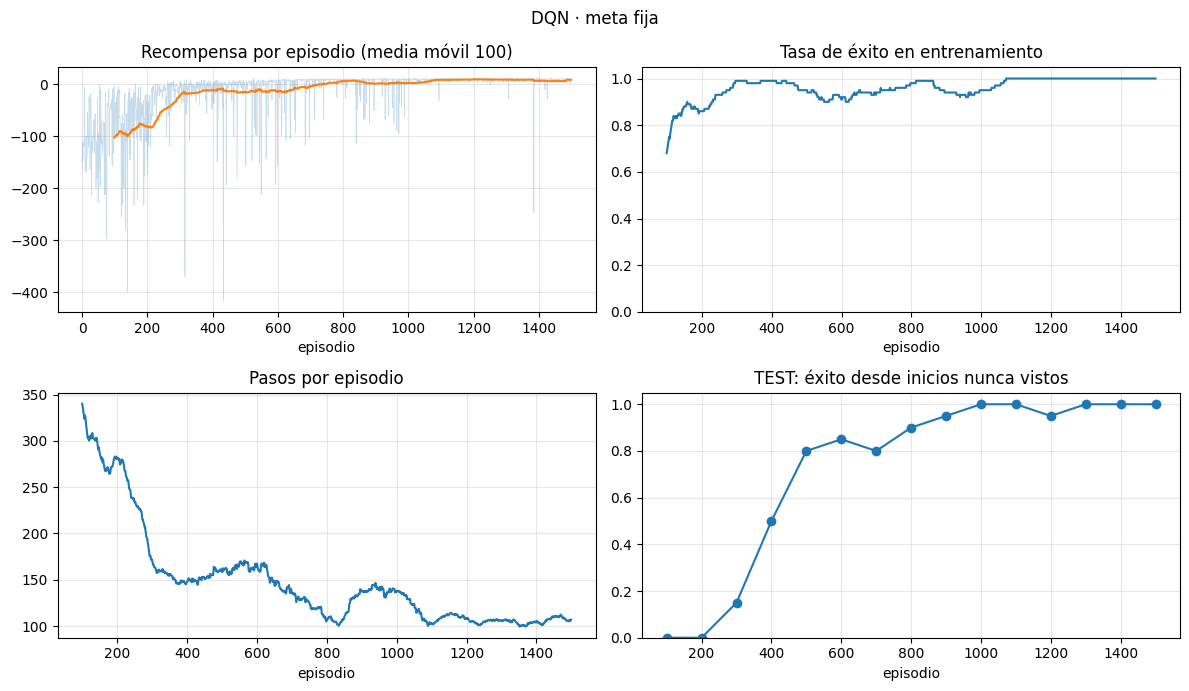
\includegraphics[width=\columnwidth]{figuras/03_curva_dqn.png}
\caption{Curva de aprendizaje de DQN con meta fija: recompensa, tasa de éxito de entrenamiento, pasos y test sobre inicios no vistos.}
\label{fig:curva}
\end{figure}

\begin{figure}[ht]
\centering
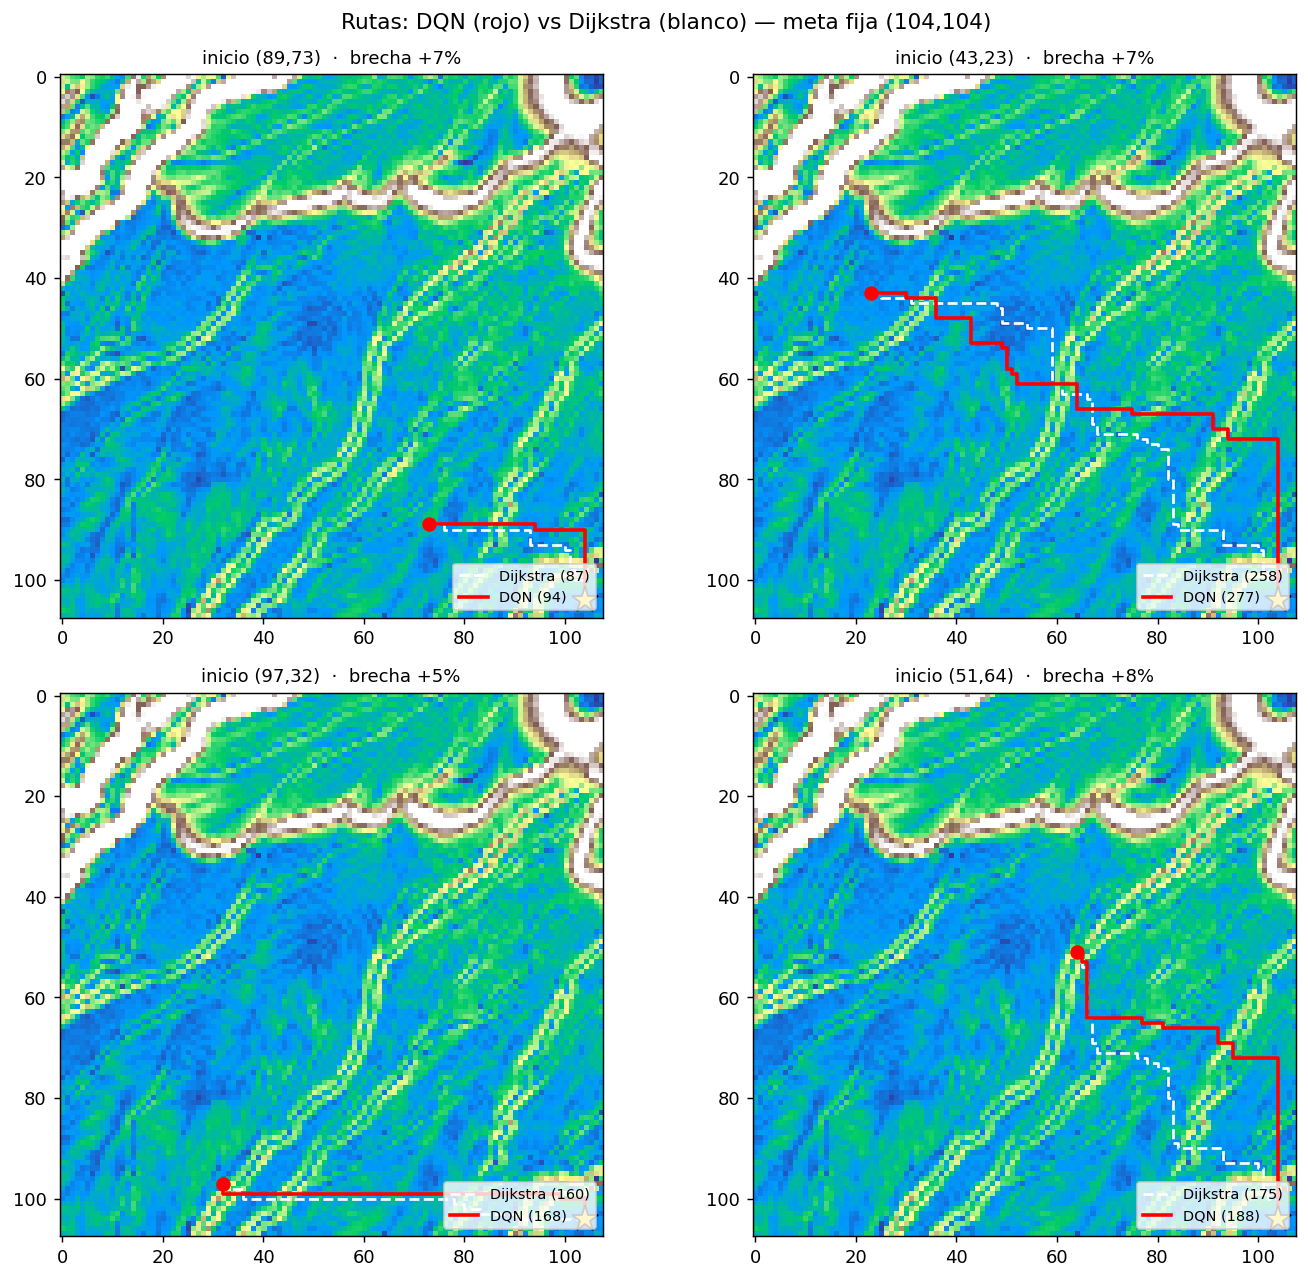
\includegraphics[width=\columnwidth]{figuras/04_rutas_dijkstra.png}
\caption{Rutas aprendidas por DQN (rojo) frente al óptimo exacto de Dijkstra (blanco), para cuatro pares inicio--meta de test.}
\label{fig:rutas}
\end{figure}

\subsection{Ablaciones}
Se realiza un estudio de ablación análogo al planteado por Liu y Zou \cite{liu2018} desactivando de forma individual los mecanismos de estabilización del algoritmo DQN (Tabla~\ref{tab:ablacion}, Fig.~\ref{fig:ablacion}). El impacto experimental de ambas exclusiones es crítico: la desactivación de la red objetivo ($\theta^-$) impide la convergencia del aprendizaje (0\,\% de éxito), comportamiento similar al obtenido al omitir el búfer de reproducción de experiencias (0\,\% de éxito). Estos resultados evidencian la complementariedad e indispensabilidad de ambos componentes. La variante Double DQN presenta un rendimiento equivalente a la versión DQN estándar (100\,\% de éxito).

\begin{figure}[ht]
\centering
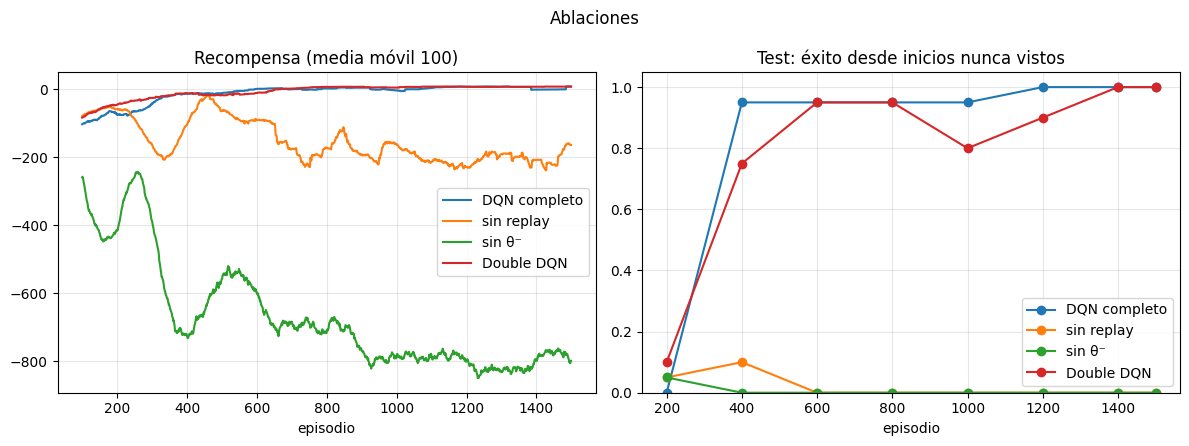
\includegraphics[width=\columnwidth]{figuras/05_ablaciones.png}
\caption{Ablaciones: DQN completo, sin \emph{replay}, sin red objetivo ($\theta^-$) y Double DQN.}
\label{fig:ablacion}
\end{figure}

\begin{table}[ht]
\caption{Ablaciones: tasa de éxito en el test}
\label{tab:ablacion}
\centering
\begin{tabular}{lc}
\toprule
Configuración & Éxito \\
\midrule
DQN completo        & 100\,\% \\
sin \emph{replay}   & 0\,\% \\
sin red objetivo ($\theta^-$) & 0\,\% \\
Double DQN          & 100\,\% \\
\bottomrule
\end{tabular}
\end{table}

\subsection{Transición estocástica}
\label{sec:estoc}
Se evalúa la robustez del agente frente a perturbaciones del entorno mediante la introducción de transiciones estocásticas (deslizamiento). Específicamente, se modela una probabilidad de deslizamiento proporcional a la pendiente local, bajo la cual la acción seleccionada es reemplazada por una dirección cardinal aleatoria. La Fig.~\ref{fig:estoc} compara el desempeño del agente en entornos deterministas frente a estocásticos. En ambas condiciones se alcanza el 100\,\% de éxito; no obstante, el entorno estocástico requiere una longitud media de trayectoria ligeramente mayor (102 pasos frente a 96). Estos resultados demuestran la adaptabilidad de la política ante incertidumbre de transición, una propiedad que la formulación clásica de Dijkstra no aborda.

\begin{figure}[ht]
\centering
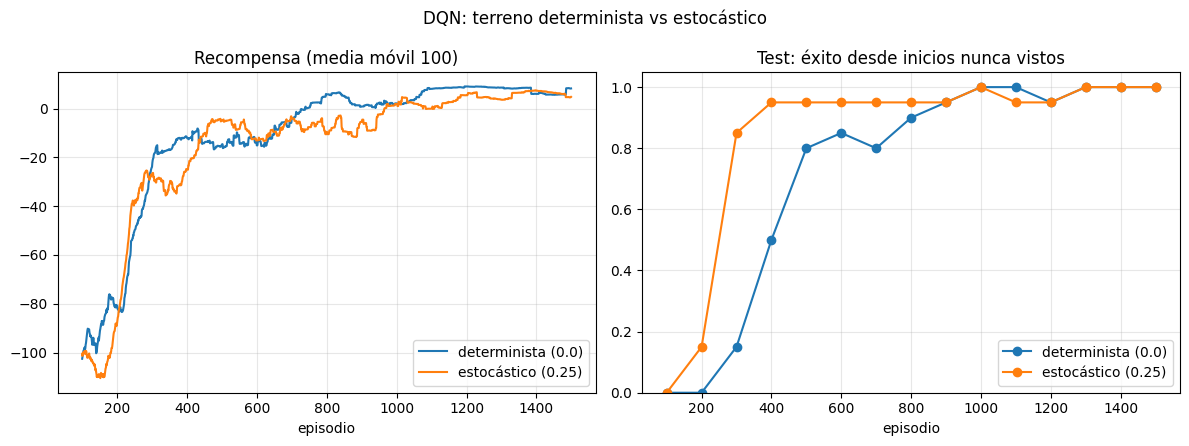
\includegraphics[width=\columnwidth]{figuras/06_estocastico.png}
\caption{DQN en terreno determinista vs estocástico (resbalón $0.25$).}
\label{fig:estoc}
\end{figure}

\subsection{Valor vs política: DQN y REINFORCE}
La comparación de desempeño entre el enfoque basado en valor (DQN) y el basado en política (REINFORCE) se presenta en la Fig.~\ref{fig:reinforce}. Ambos paradigmas alcanzan tasas de éxito elevadas (DQN: 100\,\%, REINFORCE: 95\,\%). Sin embargo, la dinámica de aprendizaje presenta diferencias sustanciales: DQN converge de forma suave y estable debido al efecto del búfer de reproducción y la red objetivo, mientras que REINFORCE exhibe una varianza significativa, con oscilaciones marcadas en el retorno episódico. Esta divergencia ilustra las características clásicas asociadas a cada familia de algoritmos.

\begin{figure}[ht]
\centering
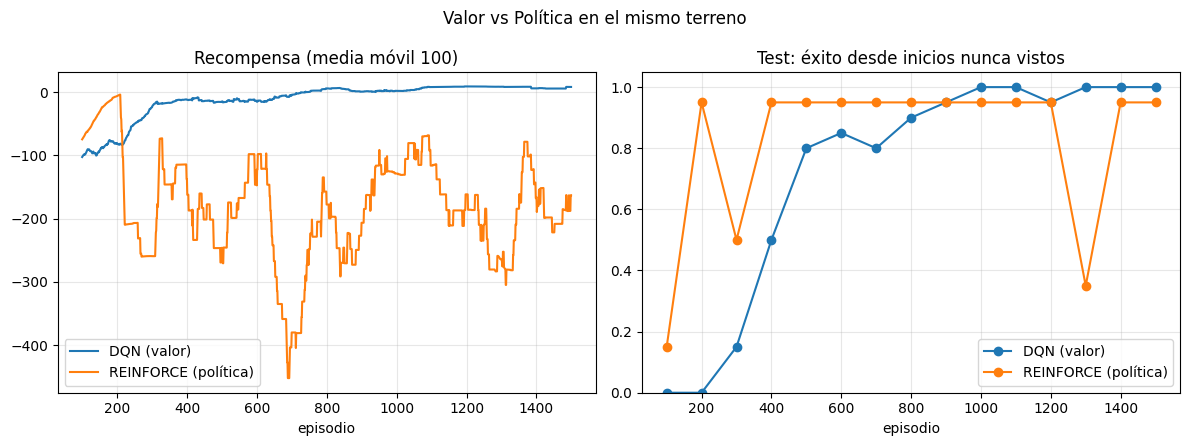
\includegraphics[width=\columnwidth]{figuras/07_dqn_vs_reinforce.png}
\caption{Valor vs política: DQN y REINFORCE en el mismo terreno.}
\label{fig:reinforce}
\end{figure}

\subsection{Divergencia con meta aleatoria}
La Fig.~\ref{fig:diverge} presenta el rendimiento de DQN ante la introducción de objetivos variables en cada episodio (configuración *goal-conditioned*). Se observa que la magnitud media de los valores $Q$ se mantiene estable hasta el episodio 1000, momento a partir del cual experimenta una divergencia asintótica, escalando de un valor de $\sim 1$ a más de $2400$. De forma simultánea, la tasa de éxito colapsa por debajo del 10\,\%. Esta inestabilidad se atribuye al sesgo de sobreestimación del operador de maximización acumulado mediante *bootstrapping*, justificando la adopción de un esquema de meta fija en el presente estudio.

\begin{figure}[ht]
\centering
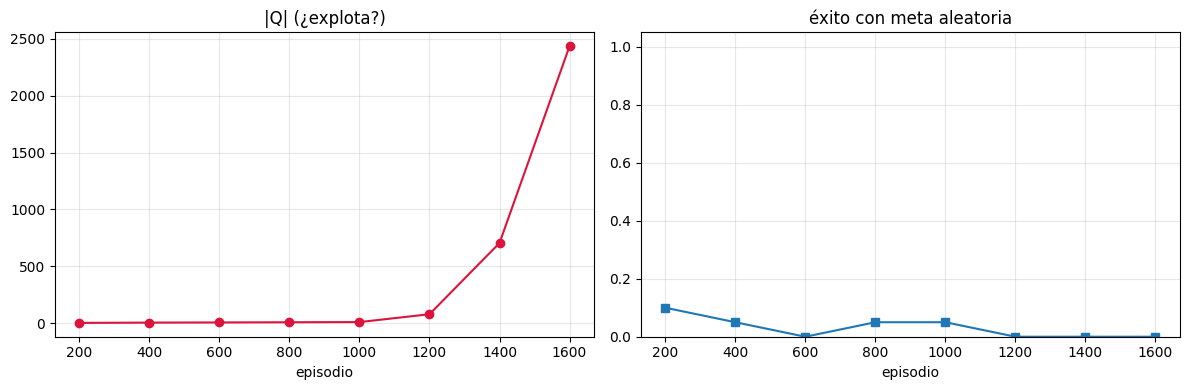
\includegraphics[width=\columnwidth]{figuras/08_divergencia.png}
\caption{Con meta aleatoria, la magnitud media de $Q$ (izq.) crece sin control (divergencia) y el éxito (der.) no se sostiene.}
\label{fig:diverge}
\end{figure}
\section{Discusión}
\label{sec:disc}

\subsection{La trampa del shaping potencial}
El rediseño de recompensa (*reward shaping*) potencial formulado bajo un factor de descuento temporal $\gamma < 1$ induce un sesgo residual positivo proporcional a la distancia al objetivo. Específicamente, al evaluar una trayectoria cíclica cerrada entre dos celdas adyacentes $X$ e $Y$ distantes de la meta, la suma de las recompensas potenciales intermedias no se anula, sino que colapsa (*telescoping*) a un valor neto de $k(1-\gamma)(d_X + d_Y) > 0$. Para distancias al objetivo elevadas, este residuo supera el costo de paso negativo del entorno, resultando en un incentivo neto positivo por oscilar indefinidamente entre celdas lejanas (efecto *ping-pong*). En consecuencia, la política codiciosa converge hacia bucles infinitos locales. El esquema de *shaping* de progreso propuesto elimina este residuo sistemático, resolviendo la anomalía. Este fenómeno ilustra cómo una propiedad teóricamente robusta (la invariancia de la política óptima en entornos sin descuento o con trayectorias finitas sin descuento) puede degradarse en la práctica debido a su interacción con el descuento episódico.

\subsection{Divergencia y la elección de meta fija}
Bajo entornos con objetivos variables, el sesgo de sobreestimación introducido por el operador $\max$ se propaga y amplifica de forma recursiva a través del proceso de *bootstrapping*, induciendo la divergencia exponencial observada de los valores $Q$. Si bien el algoritmo Double DQN ralentiza este proceso de desestabilización, no logra evitar la divergencia en la configuración evaluada. Por el contrario, la fijación del objetivo genera un campo de valores único, estacionario y convergente. Dicha restricción metodológica no representa una limitación accidental del diseño, sino una decisión fundamentada orientada a garantizar la estabilidad numérica del aprendizaje.

\subsection{Limitación: política de meta única}
La principal limitación de la política desarrollada radica en su especificidad respecto al objetivo: aunque el agente demuestra una notable capacidad de generalización sobre los estados iniciales, la política está parametrizada para una meta estática específica. Modificar la ubicación del objetivo requiere reiniciar el proceso de entrenamiento. Extender la capacidad de generalización hacia metas arbitrarias requiere el empleo de arquitecturas condicionales y mecanismos de regularización robustos contra la divergencia, aspectos propuestos como líneas prioritarias de investigación futura.

\section{Conclusiones}
\label{sec:conc}

En el presente estudio, se ha desarrollado e implementado de forma exitosa un marco experimental para la navegación autónoma de costo mínimo sobre topografía real, utilizando Aprendizaje por Refuerzo Profundo bajo condiciones de observación parcial y estados iniciales variables. A partir de los resultados cuantitativos y análisis empíricos presentados, se formulan las siguientes conclusiones:

\begin{itemize}
  \item \textbf{Generalización y Optimalidad:} El agente entrenado demostró una notable capacidad de generalización al alcanzar la meta desde configuraciones de inicio no observadas durante el entrenamiento, registrando una tasa de éxito del 100\,\%. Las trayectorias generadas exhibieron una desviación media de costo de solo el 3,3\,\% en comparación con la frontera óptima global calculada por el algoritmo de Dijkstra.
  \item \textbf{Robustez ante Incertidumbre:} Bajo transiciones estocásticas que modelan condiciones de deslizamiento físico, la política aprendida exhibió resiliencia al mantener el 100\,\% de éxito, requiriendo un incremento de solo 6 pasos en promedio respecto a la simulación determinista (102 frente a 96 pasos). Esto evidencia la adaptabilidad del DRL frente a la rigidez de la planificación clásica.
  \item \textbf{Indispensabilidad de Mecanismos en DQN:} El análisis de ablación demostró que tanto la memoria de reproducción de experiencias como la red objetivo congelada ($\theta^-$) son mecanismos críticos para la estabilidad numérica del aprendizaje. La desactivación individual de cualquiera de ellos provocó el colapso del entrenamiento, resultando en una tasa de éxito del 0\,\%.
  \item \textbf{Sensibilidad al Diseño de Recompensas:} Se caracterizó empíricamente que el rediseño potencial tradicional ($F = \gamma \Phi(s') - \Phi(s)$) induce comportamientos espurios (bucles infinitos locales) en trayectorias extensas cuando se opera con factores de descuento $\gamma < 1$. Por el contrario, el esquema de recompensa por progreso propuesto resolvió esta inestabilidad al eliminar los residuos acumulados en ciclos cerrados.
  \item \textbf{Inestabilidad ante Objetivos Variables:} Se demostró que la formulación estándar de DQN es propensa a la divergencia asintótica de los valores $Q$ (escalando de $\sim 1$ a más de $2400$) ante metas aleatorias, debido a la realimentación del sesgo del operador $\max$. Esto justifica de manera metodológica la adopción de una política parametrizada para un objetivo estacionario en el presente trabajo.
\end{itemize}

% --------------------------------------------------------------------------
\begin{thebibliography}{11}
\bibitem{dijkstra1959} E. W. Dijkstra, ``A note on two problems in connexion with
graphs,'' \emph{Numerische Mathematik}, vol.~1, pp.~269--271, 1959.
\bibitem{mnih2015} V. Mnih \emph{et al.}, ``Human-level control through deep
reinforcement learning,'' \emph{Nature}, vol.~518, pp.~529--533, 2015.
\bibitem{vanhasselt2016} H. van Hasselt, A. Guez, and D. Silver, ``Deep
reinforcement learning with double Q-learning,'' in \emph{AAAI}, 2016.
\bibitem{liu2018} R. Liu and J. Zou, ``The effects of memory replay in
reinforcement learning,'' in \emph{Allerton Conf.}, IEEE, 2018.
\bibitem{ng1999} A. Ng, D. Harada, and S. Russell, ``Policy invariance under reward
transformations: theory and application to reward shaping,'' in \emph{ICML}, 1999.
\bibitem{williams1992} R. J. Williams, ``Simple statistical gradient-following
algorithms for connectionist reinforcement learning,'' \emph{Machine Learning},
vol.~8, pp.~229--256, 1992.
\bibitem{mnih2016} V. Mnih \emph{et al.}, ``Asynchronous methods for deep
reinforcement learning,'' in \emph{ICML}, 2016.
\bibitem{sutton2018} R. S. Sutton and A. G. Barto, \emph{Reinforcement Learning: An
Introduction}, 2nd ed. MIT Press, 2018.
\bibitem{schaul2015} T. Schaul, D. Horgan, K. Gregor, and D. Silver, ``Universal
value function approximators,'' in \emph{ICML}, 2015.
\bibitem{schaul2016} T. Schaul, J. Quan, I. Antonoglou, and D. Silver, ``Prioritized
experience replay,'' in \emph{ICLR}, 2016.
\bibitem{andrychowicz2017} M. Andrychowicz \emph{et al.}, ``Hindsight experience
replay,'' in \emph{NeurIPS}, 2017.
\end{thebibliography}

% --------------------------------------------------------------------------
% % Figuras del informe (flotan al inicio de columna/página).
\begin{figure}[t]
\centering
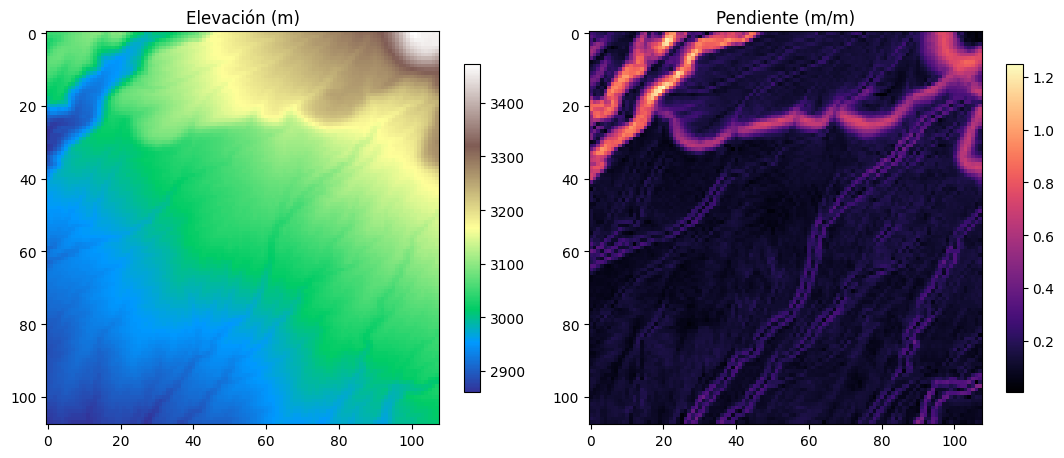
\includegraphics[width=\columnwidth]{figuras/01_terreno.png}
\caption{Terreno real (faldas del Misti): elevación (izq.) y pendiente (der.),
malla $108\times108$ de 30~m.}
\label{fig:terreno}
\end{figure}

\begin{figure}[t]
\centering
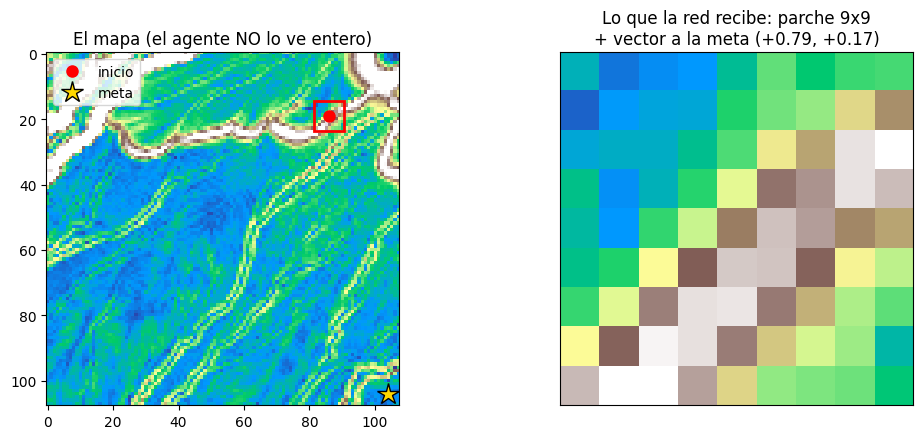
\includegraphics[width=\columnwidth]{figuras/02_observacion.png}
\caption{Observación local: el mapa completo con la ventana del agente (izq.) y el
parche $9\times9$ que recibe la red (der.), más el vector a la meta.}
\label{fig:obs}
\end{figure}

\begin{figure}[t]
\centering
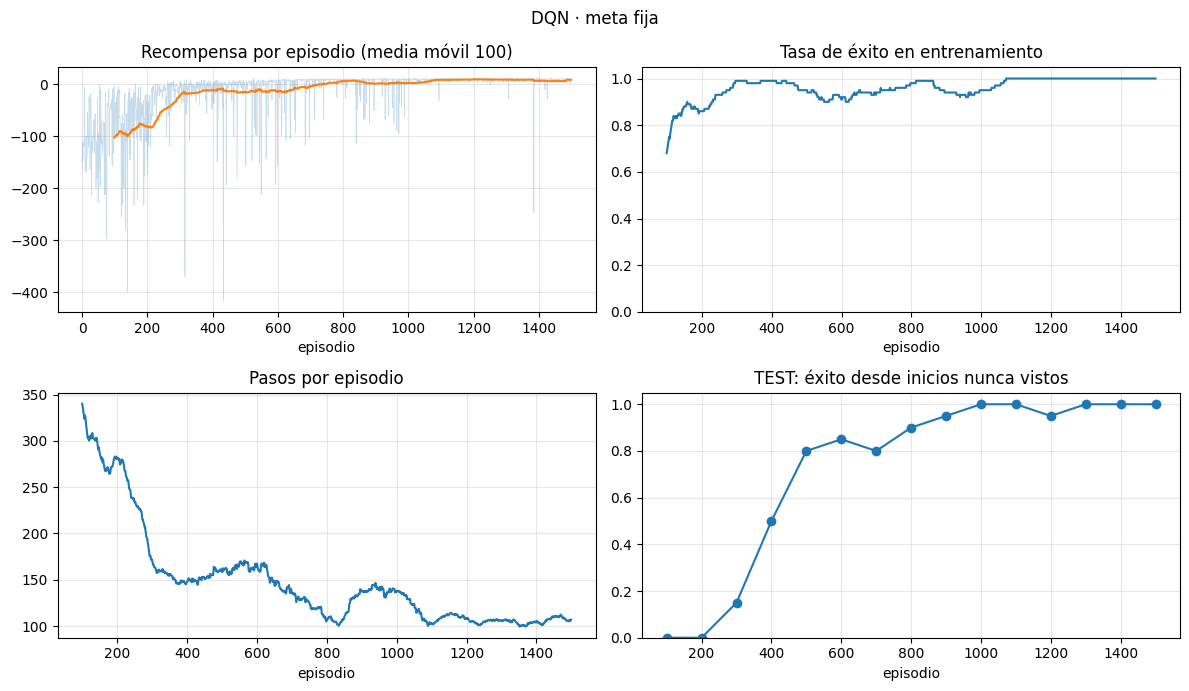
\includegraphics[width=\columnwidth]{figuras/03_curva_dqn.png}
\caption{Curva de aprendizaje de DQN con meta fija: recompensa, tasa de éxito de
entrenamiento, pasos y test sobre inicios no vistos.}
\label{fig:curva}
\end{figure}

\begin{figure}[t]
\centering
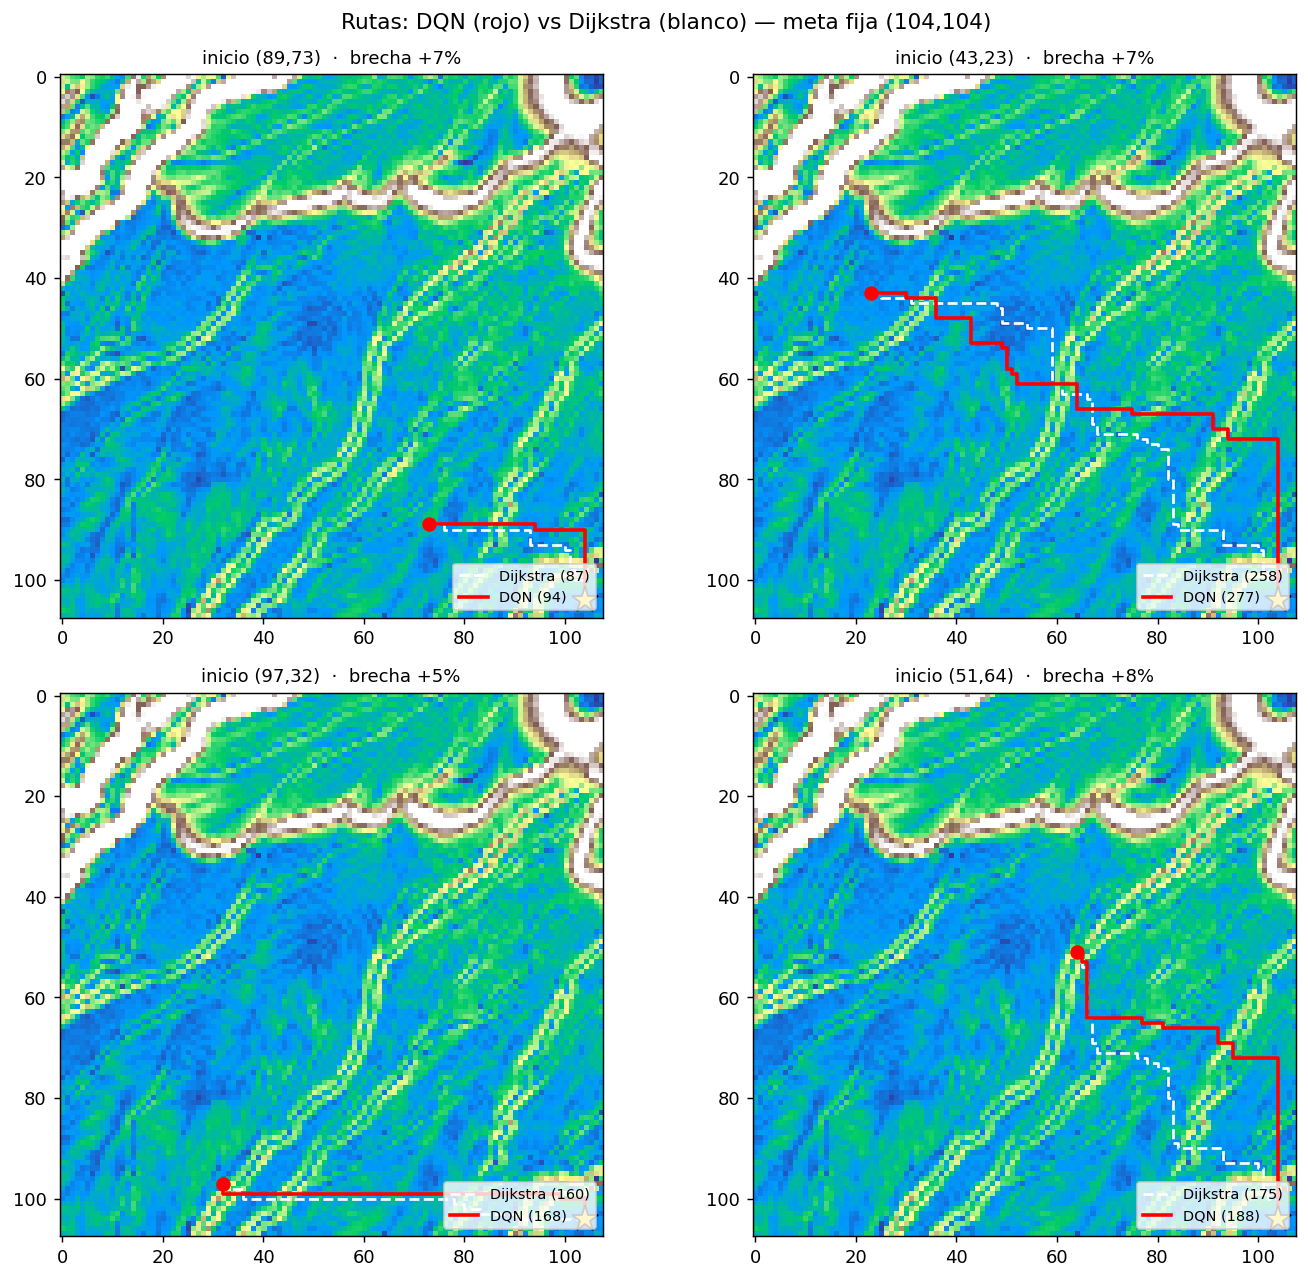
\includegraphics[width=\columnwidth]{figuras/04_rutas_dijkstra.png}
\caption{Rutas aprendidas por DQN (rojo) frente al óptimo exacto de Dijkstra
(blanco), para cuatro pares inicio--meta de test.}
\label{fig:rutas}
\end{figure}

\begin{figure}[t]
\centering
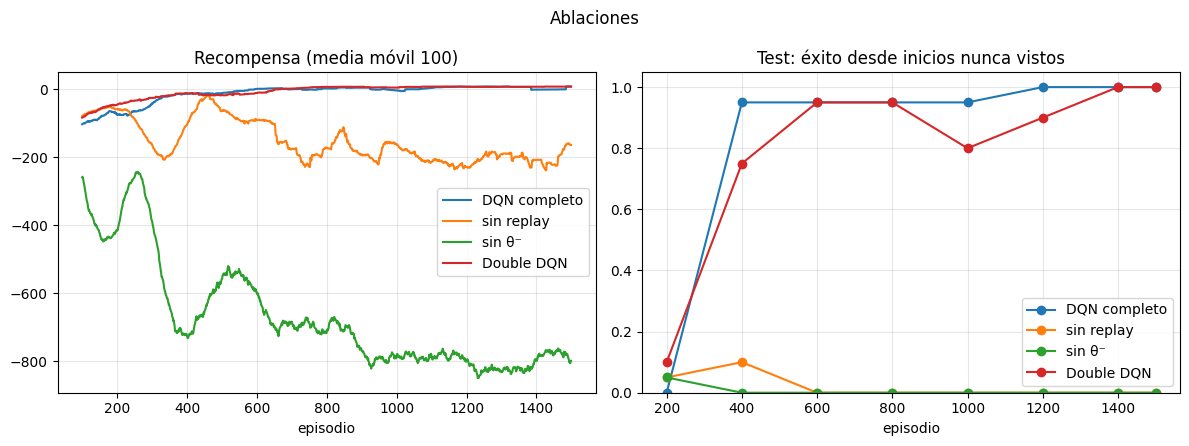
\includegraphics[width=\columnwidth]{figuras/05_ablaciones.png}
\caption{Ablaciones: DQN completo, sin \emph{replay}, sin red objetivo
($\theta^-$) y Double DQN.}
\label{fig:ablacion}
\end{figure}

\begin{figure}[t]
\centering
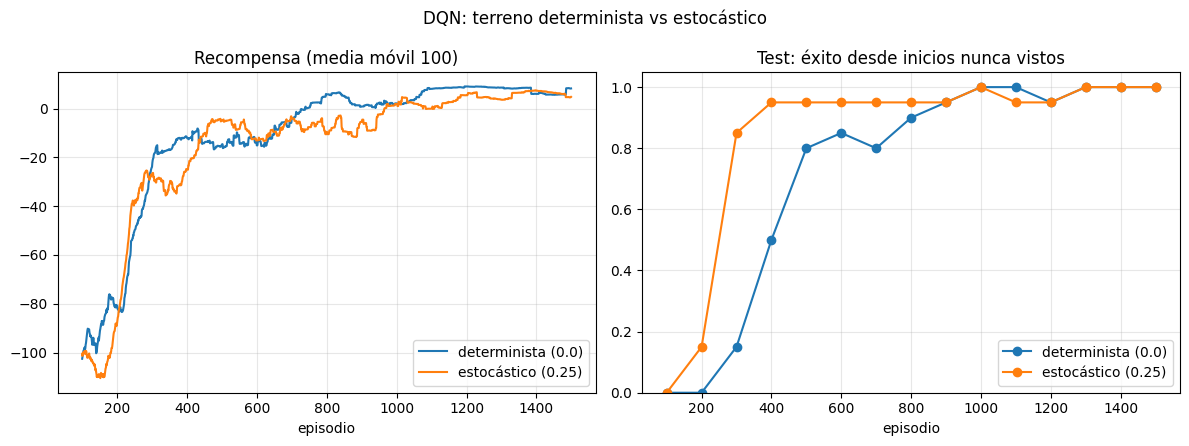
\includegraphics[width=\columnwidth]{figuras/06_estocastico.png}
\caption{DQN en terreno determinista vs estocástico (resbalón $0.25$).}
\label{fig:estoc}
\end{figure}

\begin{figure}[t]
\centering
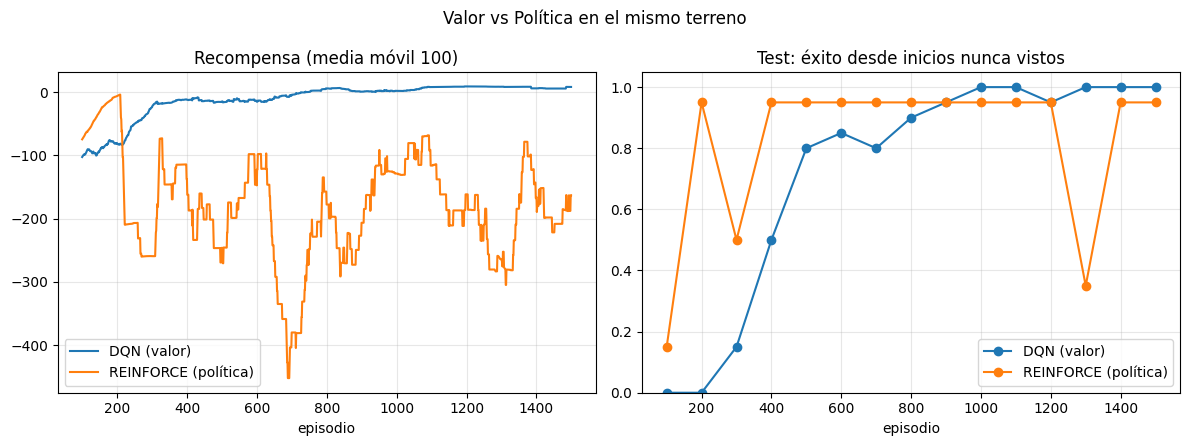
\includegraphics[width=\columnwidth]{figuras/07_dqn_vs_reinforce.png}
\caption{Valor vs política: DQN y REINFORCE en el mismo terreno.}
\label{fig:reinforce}
\end{figure}

\begin{figure}[t]
\centering
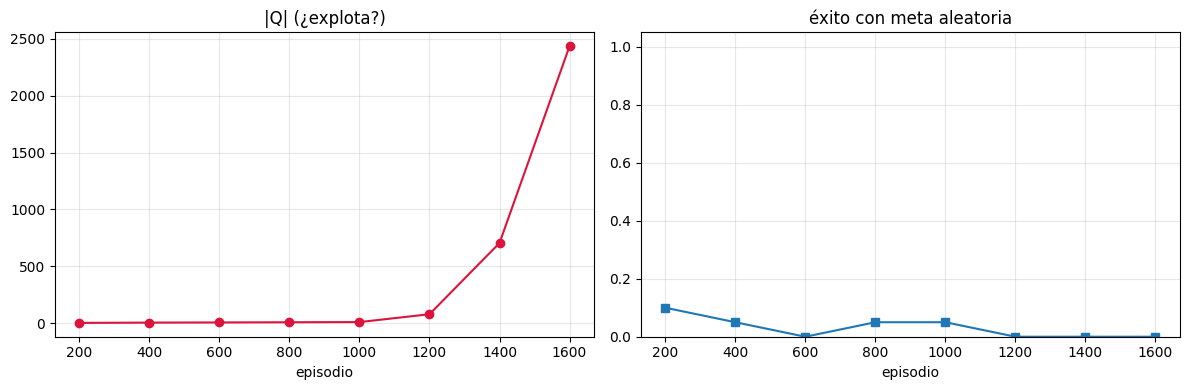
\includegraphics[width=\columnwidth]{figuras/08_divergencia.png}
\caption{Con meta aleatoria, la magnitud media de $Q$ (izq.) crece sin control
(divergencia) y el éxito (der.) no se sostiene.}
\label{fig:diverge}
\end{figure}


\end{document}
